\documentclass[presentation]{beamer}   % to compile the presentation
%\documentclass[handout]{beamer}        % to compile 2x2 handouts
\usepackage[ansinew]{inputenc}
\usepackage[T1]{fontenc}
\usepackage{lmodern,textcomp}
\usepackage{breakurl}
\usepackage{graphicx}

\usetheme{Algo}
%\usetheme{Warsaw}

\usepackage[formats]{listings}
\lstdefineformat{C}{% 
	\{=\newline\string\newline\indent,% 
	\}=[;]\newline\noindent\string\newline,% 
	\};=\newline\noindent\string\newline,% 
	;=[\ ]\string\space}
\lstset{language=C}

%\usepackage{/usr/lib64/R/share/texmf/Sweave}
%\usepackage{/Library/Frameworks/R.framework/Resources/share/texmf/Sweave}
\setbeamercovered{transparent}
\AtBeginSection[]
        {
                \begin{frame}<beamer>
                        \frametitle{}
                        \tableofcontents[currentsection]
                \end{frame}
        }

\begin{document}
\pgfdeclareimage[height=1cm]{Biglogo}{dtu_logo}
%\pgfdeclareimage[width=12mm]{footlogo}{partek_logo_s}

\author{Sigmar Stef\`{a}nson and Francesco Favero}
\title[PSSM,ANN,SVM]{Comparison of MHC peptide binding data classification using PSSM, SVM and ANN}
\date{15 Dic. 2010}
\titlegraphic{\pgfuseimage{Biglogo}} % Graphics for title slide
%\logo{\pgfuseimage{footlogo}} % The left logo



\begin{frame}
  \maketitle
\end{frame}

\begin{frame}
  \frametitle{Outline}
  \tableofcontents[currentsection]
\end{frame}

<<<<<<< HEAD
\begin{frame}
  \frametitle{Methods}
  \begin{itemize}
    \item<1> We looked at three methods from the class used for MHC peptide binding prediction.
    \item<2>  The Position specific scoring matrix (PSSM), Support vector machines (SVM) and Artificial neural networks (ANN).
    \item<3> Generating PSSM weight matrix just uses data from positive binders (> 0.426 binding coefficient)
    \item<4> The other two, SVM and ANN are machine learning methods, non-binders also useful.
    \item<5> Pearsons correlation coefficient to evaluate the predictive performance of the methods.
    \item<6> its invariant in terms of location and scale and should therefore be ideal comparing different methods.
	\begin{equation}
		pcc = \frac{ \sum_n{(x-x_m)(y-y_m) } }{ \sqrt{ \sum_n{(x-x_m)^2}\cdot\sum_{n}{(y-y_m)^2} } }
	\end{equation}
  \end{itemize}
\end{frame}

\begin{frame}
  \frametitle{Data}
  \begin{itemize}
    \item<1> All 35 MHC datasets from course used in PSSM and ANN.
    \item<2>  Looked specifically into datasets containing relatively few binders (B4001) to stress the difference between methods using and not using non-binding data.
  \end{itemize}
\end{frame}

\section{PSSM}
\begin{frame}
 \frametitle{PSSM (PWM)}
 \begin{columns}
  \begin{column}{5cm}
   \begin{block}\centering
    PSSM is used to represent a motif pattern.
    Is a good method to estimate the relevance 
    of the position of an aminoacids in a MHC binding. 
   \end{block}
   \pause
   \begin{block}\centering
   Uses \textit{Pseudo Counts} when few data are available:
    \begin{equation}
     p_a = \frac{\alpha \cdot f_a + \beta \cdot g_a}{\alpha + \beta}
    \end{equation}
   \end{block}
   \pause
  \end{column}
  \begin{column}{5cm}
   \begin{block}\centering
    \textit{Sequence Weighting} can be used to reduce redoundancy:
    \begin{equation}
     w_{k} = \sum_{p}{\frac{1}{r_p \cdot s_p}}
    \end{equation}

   \end{block}
   \pause
   \begin{block}\centering
   
   \end{block}
  
  
  \end{column}
 \end{columns}

\end{frame}

\section{SVM}
\begin{frame}

\end{frame}

\section{ANN}
\begin{frame}

\end{frame}

\section{Results}
\begin{frame}

\end{frame}

\subsection{PSSM}
\begin{frame}
\begin{figure*}[ht]
\begin{center}
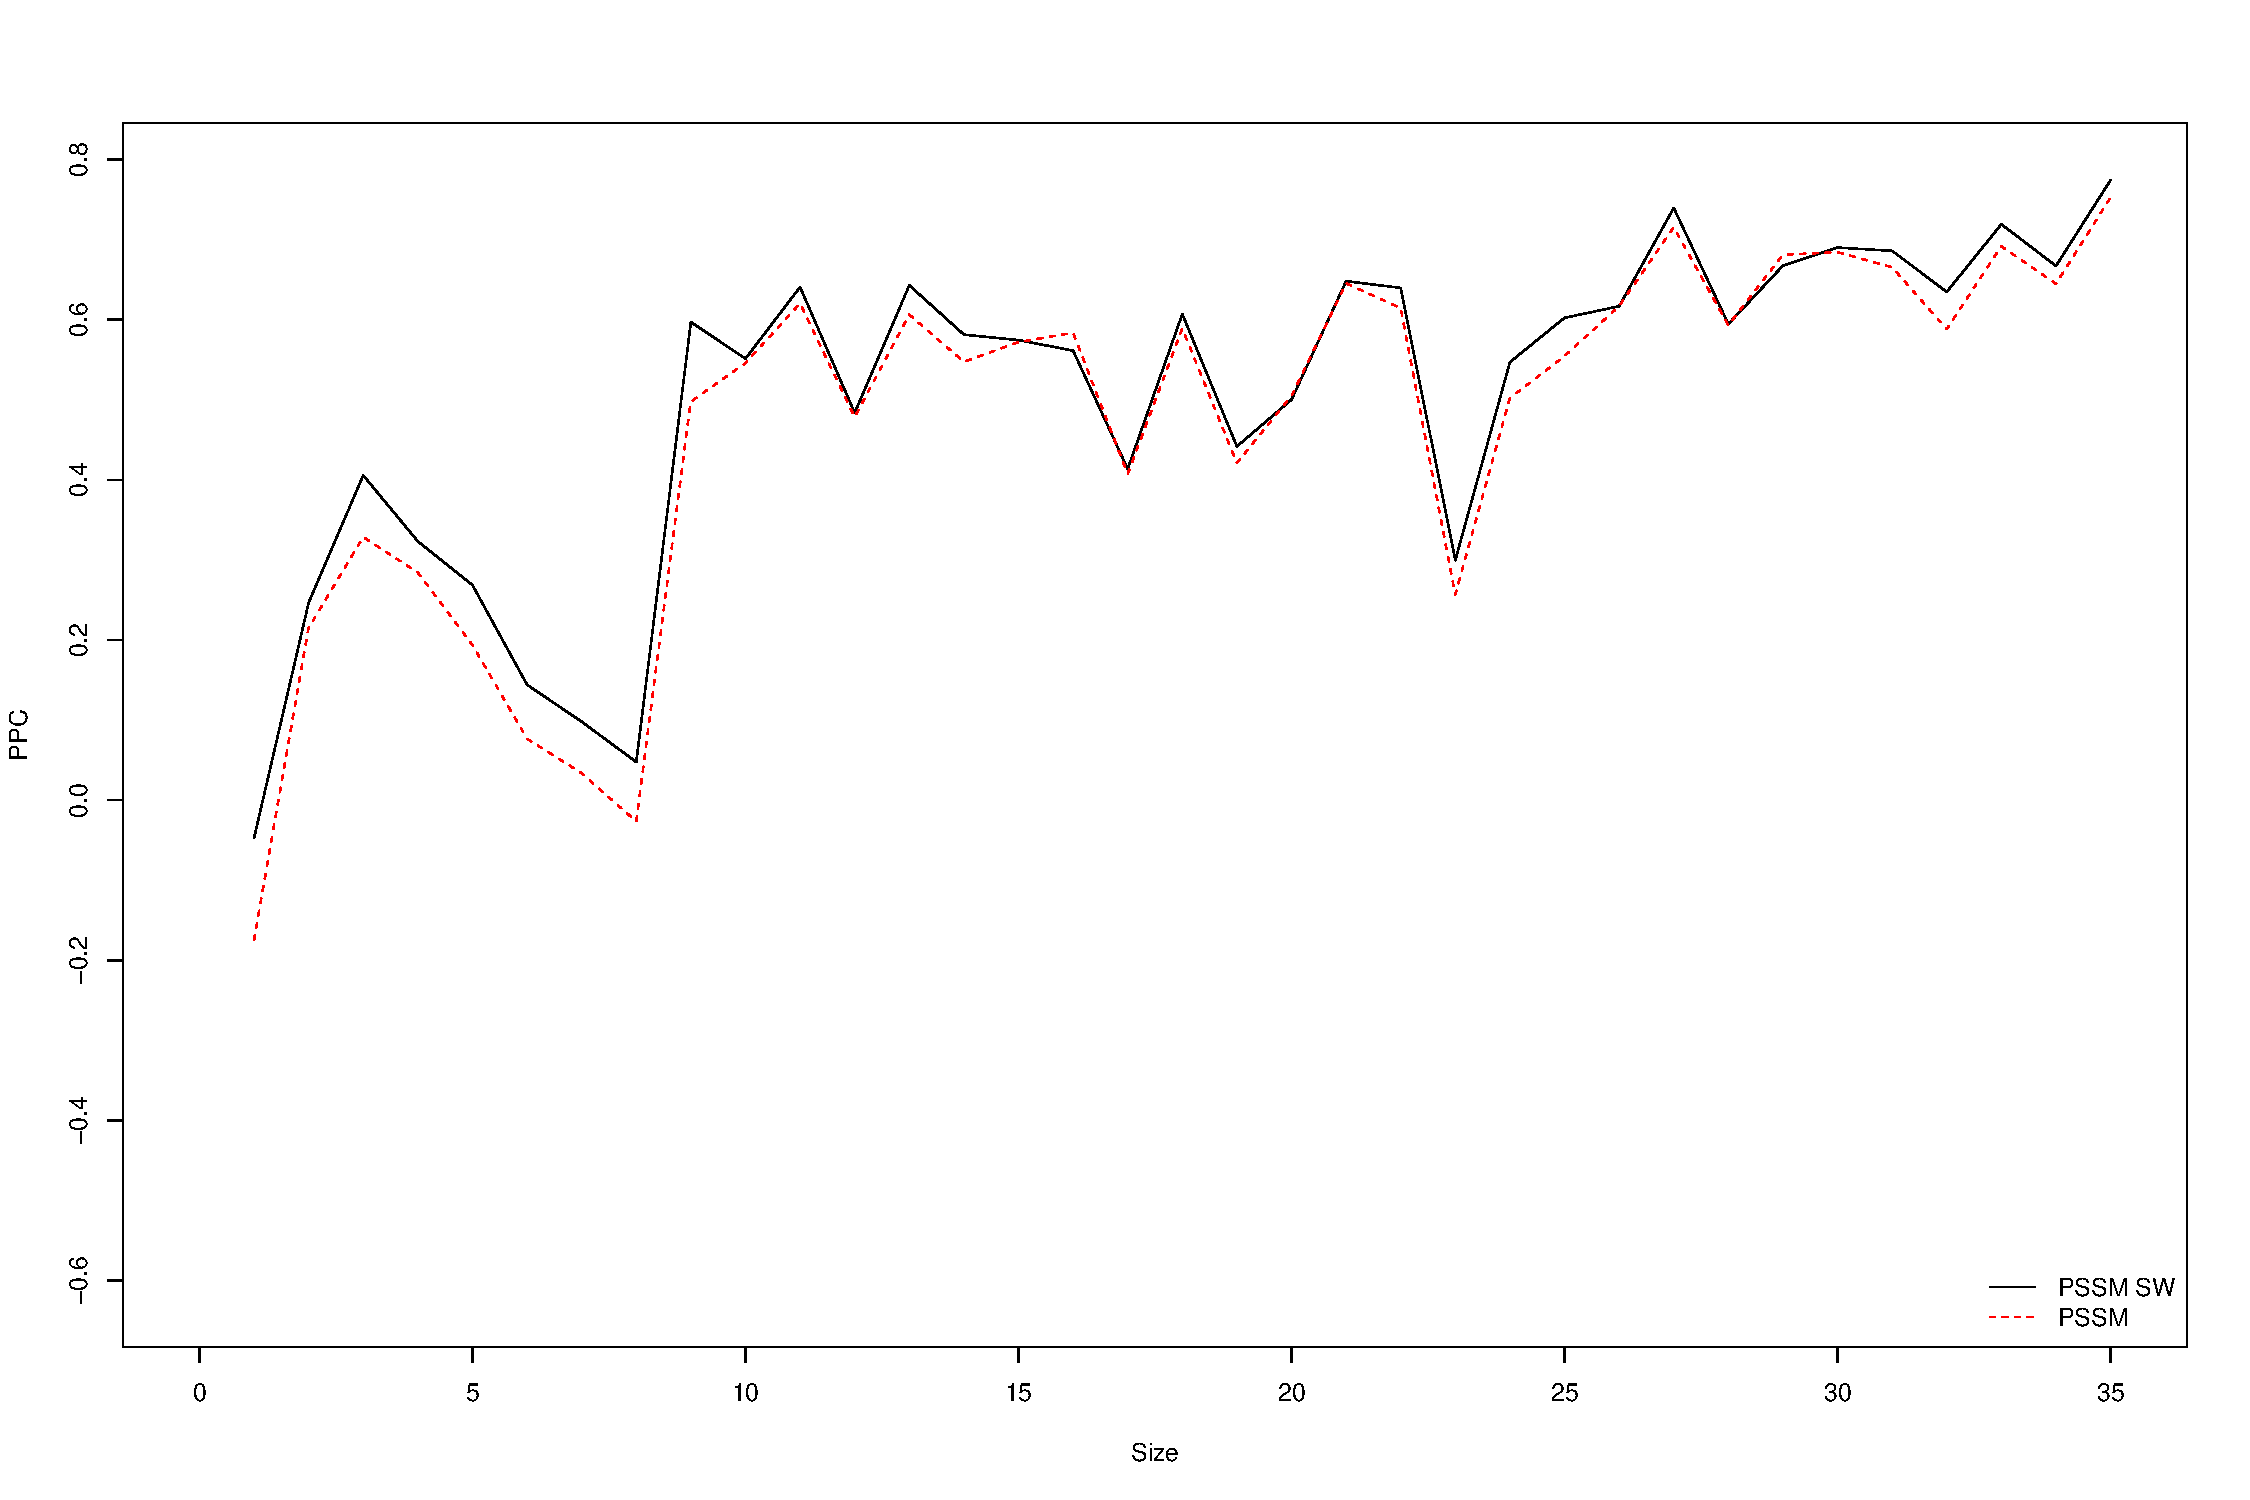
\includegraphics[width=18cm]{fig/pssmLN1.pdf}
\caption{Plot of the average Pearson Correlation Coefficient of the 5 test for the PSSM algorithm on each of the 35 alleles. The alleles are ordered by the size of the dataset, the order is the following:
B5701, A3002, A2301, B4501, B1801, B4002, B4403, B4402, A2902, A2402, B5101, A2403, B5301, B5401, A3001, A2601, B0801, B3501, A6901, B2705, B1501, B5801, B4001, A6801, A3301, A0101, B0702, A6802, A0206, A0203, A0202, A3101, A1101, A0301 and A0201.}\label{fig:pssm1}
\end{center}
\end{figure*}
\item<1> Using sequence weighting providest better results in most cases.
\item<2> The B4001 clearly visible, large dataset, low number of binders, PCC just over 0.3
\item<3> Small datasets provide PSSM with good prediction performance, pseudo counts helps.
\end{frame}

\subsection{SVM}
\begin{frame}

\end{frame}

\subsection{ANN}
\begin{frame}

\end{frame}

\end{document} 
